\begin{theorem}
The equation of a conic with directrix $\vec{n}^{\top}\vec{x} = c$, eccentricity $e$ and focus $\vec{F}$ is given by 
\begin{align}
    \label{2/31/eq:conic_quad_form}
    \vec{x}^{\top}\vec{V}\vec{x}+2\vec{u}^{\top}\vec{x}+f=0
    \end{align}
where     
\begin{align}
\label{2/31/eq:conic_quad_form_v}
\vec{V} &=\norm{\vec{n}}^2\vec{I}-e^2\vec{n}\vec{n}^{\top}, \\
\label{2/31/eq:conic_quad_form_u}
\vec{u} &= ce^2\vec{n}-\norm{\vec{n}}^2\vec{F}, \\
\label{2/31/eq:conic_quad_form_f}
f &= \norm{\vec{n}}^2\norm{\vec{F}}^2-c^2e^2
\end{align}
For $\abs{\vec{V}}>0$, the equation represents an ellipse, while for $\abs{\vec{V}}<0$, the equation represents a hyperbola.
\end{theorem}
\begin{theorem}
For $\abs{\vec{V}} \ne 0$ the equations of minor and major axes of the conic in \eqref{2/31/eq:conic_quad_form} are given by
\begin{align}
    \vec{p_i}^{\top}(\vec{x}-\vec{c})&=0,i=1,2\label{2/31/eq:minmaj}
\end{align}
\end{theorem}
\begin{theorem}
The eccentricity of the conic in \eqref{2/31/eq:conic_quad_form} is given by
\begin{align}
e= \sqrt{1-\frac{\lambda_1}{\lambda_2}}
\label{2/31/eq:e}
\end{align}
\end{theorem}
\begin{definition}[Latus rectum]
The latus rectum of a conic section is the chord (line segment) that passes through the focus, is perpendicular to the major axis and has both endpoints on the curve.
\end{definition}
\begin{theorem}
The equation latus rectum of the conic in \eqref{2/31/eq:conic_quad_form} is given by
\begin{align}
    \vec{n}^{\top}\brak{\vec{x}-\vec{F}} = 0
    \label{2/31/eq:lreq}
\end{align}
\end{theorem}
\begin{theorem}
For $\abs{\vec{V}} \ne 0$, the lengths of semi-major and semi-minor axes of the conic in \eqref{2/31/eq:conic_quad_form} are 
\begin{align} 
\sqrt{\frac{\vec{u}^{\top}\vec{V}^{-1}\vec{u} -f}{\lambda_1}}, 
\sqrt{\bigg | \frac{f-\vec{u}^{\top}\vec{V}^{-1}\vec{u}}{\lambda_2}\bigg | }
\label{2/31/eq:ab}
\end{align} 
\end{theorem}
% \begin{theorem}
% For $\abs{\vec{V}} \ne 0$ the foci of the conic in \eqref{2/31/eq:conic_quad_form} are given by
% \begin{align}
%   \vec{F} &=\vec{c}\pm\brak{\sqrt{\frac{(\vec{u}^T\vec{V}^{-1}\vec{u}-f)(\lambda_2-\lambda_1)}{\lambda_1\lambda_2}}}\vec{p_1} \label{2/31/eq:foci}
% \end{align}
% \end{theorem}
\begin{theorem}
For $\abs{\vec{V}} \ne 0$, the length of latus rectum (LLR) of the conic in \eqref{2/31/eq:conic_quad_form} is given by 
\begin{align} 
LLR=\dfrac{2\bigg | \dfrac{f-\vec{u}^{\top}\vec{V}^{-1}\vec{u}}{\lambda_2}\bigg | }{{\sqrt{\dfrac{\vec{u}^{\top}\vec{V}^{-1}\vec{u} -f}{\lambda_1}}}}
\label{2/31/eq:LLR}
\end{align} 
\end{theorem}
\begin{proof}
Using \eqref{2/31/eq:ab}, we can write
\begin{align}
  \vec{F} &=\vec{c}\pm\brak{\sqrt{\frac{(\vec{u}^T\vec{V}^{-1}\vec{u}-f)(\lambda_2-\lambda_1)}{\lambda_1\lambda_2}}}\vec{p_1} \label{2/31/eq:foci}
\end{align}
Also, we know, for $\abs{\vec{V}} \ne 0$,
\begin{align}
    \vec{n}=\sqrt{\lambda_2}\vec{p_1} \label{2/31/eq:conv}\\
    \Rightarrow \vec{p_1}^{\top}\brak{\vec{x}-\vec{F}} = 0
\end{align}
is the equation of latus rectum. Solving this with \eqref{2/31/eq:conic_quad_form} and simplifying, we get 
\begin{align}
    \vec{H}=\vec{F}\pm\sqrt{\lambda_1\brak{ \dfrac{\vec{u}^{\top}\vec{V}^{-1}\vec{u} -f}{\lambda_2^2}}} \vec{p_2}
\end{align}
as the points of intersection. Hence, the length of line segment is
\begin{align}
    LLR=\bigg |\bigg |2\sqrt{\lambda_1\brak{ \dfrac{\vec{u}^{\top}\vec{V}^{-1}\vec{u} -f}{\lambda_2^2}}} \vec{p_2}\bigg |\bigg |=\dfrac{2\bigg | \dfrac{f-\vec{u}^{\top}\vec{V}^{-1}\vec{u}}{\lambda_2}\bigg | }{{\sqrt{\dfrac{\vec{u}^{\top}\vec{V}^{-1}\vec{u} -f}{\lambda_1}}}}
\end{align}
\end{proof}
Given, length of latus rectum is 36 and focii are $\myvec{0\\ \pm12}$. Let us consider $\myvec{0\\ 12}$ for solving the problem.
\begin{align}
    \vec{F} =\myvec{0\\ 12}\Rightarrow\norm{\vec{F}}=12
\end{align}
Let $\vec{u}^{\top}\vec{V}^{-1}\vec{u}-f=\alpha$. From \eqref{2/31/eq:ab},\eqref{2/31/eq:e},\eqref{2/31/eq:LLR}
\begin{align}
    \sqrt{\dfrac{\alpha}{\lambda_1}}\sqrt{1-\frac{\lambda_1}{\lambda_2}}=12\label{2/31/eq:one}\\
    \dfrac{2\brak{\dfrac{-\alpha}{\lambda_2}}}{\sqrt{\dfrac{\alpha}{\lambda_1}}}=36\label{2/31/eq:two}
\end{align}
Dividing \eqref{2/31/eq:one} by \eqref{2/31/eq:two} gives
\begin{align}
    \dfrac{\lambda_1}{\lambda_2}&=-3\\
    \Rightarrow e&=2\label{2/31/eq:q}\\
    \Rightarrow \sqrt{\frac{\alpha}{\lambda_1}}&=6\label{2/31/eq:w}
\end{align}
The associated directrix is perpendicular to the y-axis and passes through the point
\begin{align}
\myvec{0\\\sqrt{\dfrac{\alpha}{e^2\lambda_1}}}=\myvec{0\\3}
\end{align}
Hence, its equation is
\begin{align}
    \myvec{0&1}\brak{\vec{x}-\myvec{0\\3}} &= 0\\
    \Rightarrow \myvec{0&1}\vec{x} &= 3
\end{align}
Comparing it with $\vec{n}^{\top}\vec{x} = c$
\begin{align}
    \vec{n} = \myvec{0\\1}, c = 3\Rightarrow \norm{\vec{n}} = 1
\end{align}
Calculating $\vec{V}, \vec{u}$ and $f$,
\begin{align}
    \vec{V}&=1^2\myvec{1&0\\0&1} - 2^2\myvec{0\\1}\myvec{0&1}\\
    &=\myvec{1&0\\0&1}-\myvec{0&0\\0&4}=\myvec{1&0\\0&-3}\\
    \vec{u}&= 3(2^2)\myvec{0\\1} - 1^2\myvec{0\\12}=\myvec{0\\0}\\
    f &= 1^2(12^2) - 3^2(2^2)= 108
\end{align}
Hence, the required equation is
\begin{align}
    \vec{x}^{\top}\myvec{1&0\\0&-3}\vec{x}+108=0
\end{align}
Also, from \eqref{2/31/eq:lreq}, the equations of latus rectum is
\begin{align}
    \myvec{0&1}\brak{\vec{x}-\myvec{0\\12}} &= 0\\
    \Rightarrow \myvec{0&1}\vec{x} &= 12
\end{align}
Similarly, the equations of directrix and latus rectum associated with $\myvec{0\\ -12}$ are given by
\begin{align}
    \myvec{0&1}\vec{x} &= -3\\
    \myvec{0&1}\vec{x} &= -12
\end{align}
\begin{figure}[!h]
 \centering
 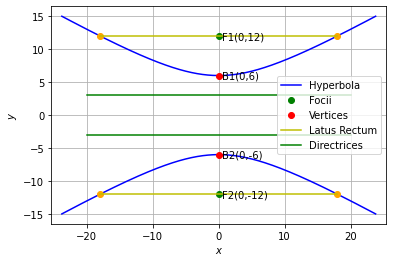
\includegraphics[width=\columnwidth]{solutions/oct/2/31/figures/Assignment5.png}
 \caption{Hyperbola}
 \label{2/31/plot}
\end{figure}
